\documentclass[12pt,fleqn]{article}\usepackage{../common}
\begin{document}
Ders 17

Onceki derste 

\[ \int \int (1-x^2-y^2) dA \]

\[ x^2+y^2 \le 1 \]

\[ x,y \ge 0 \]

entegralini hesapladik, fakat kullandigimiz yontem biraz karmasikliga yol
acti. Daha iyi bir yontem kutupsal forma gecmektir. 

Hatirlarsak $x,y$ kordinat sisteminde cift entegral icin entegrasyon
alanini yatay, dikey sekilde parcalara ayirmistik, $dA = dy \ dx$ haline
gelmisti. Kutupsal formda 

\[ \int \int  ... \ dr \ d\theta\]

seklinde bir form olur, once $r$ uzerinden entegrasyon en kolayi. Bu
demektir ki $\theta$'yi sabitleriz, ve $r$ uzerinde hareket ederiz. 

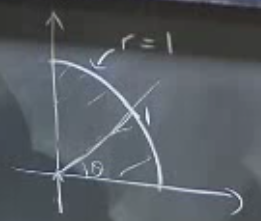
\includegraphics[height=3cm]{17_1.png}

Birim disk orneginde bu hareket basit, $r=0$'dan baslanir, ve 1 degerine
gelinceye kadar hareket edilir. $\theta$ icin 0'dan baslanir, ustteki alana
gore, $\pi/2$'ya gelinceye kadar hareket edilir. Sinirlar soyle olur:

\[ \int_0^{\pi/2} \int_0^1  ... \ dr \ d\theta\]

Fakat, dikkat, bu onemli bir nokta, $dA$ buyuklugu $dr \ d\theta$'ya esit
{\em degildir}. 

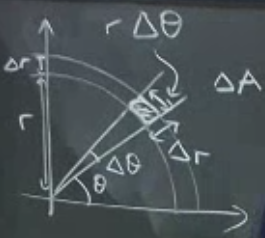
\includegraphics[height=3cm]{17_2.png}

Ustteki resimdeki ici karalanmis ufak dikdortgeni dusunelim, dikdortgenin
kenarlarindan biri biraz egimlidir (cemberin parcasi oldugu icin) fakat
kenarlar kuculdukce bu ufak alan dikdortgen olarak gorulebilir. Neyse,
kenarlarin biri $\Delta r$ (bu kolay), digeri? Oteki kenar $\Delta \theta$
degil, cunku o kenar cemberin bir parcasi, o zaman $r \ \Delta \theta$.

Bu demektir ki kenarlari sonsuz kuculttugumuz zamanda bile 

\[ dA = r \ dr \ d\theta \]

olacak. Entegral

\[ \int_0^{\pi/2} \int_0^1  f \ dr \ d\theta\]

\[ f =  (1-x^2-y^2)\]

Kutupsal forma tabii ki mekanik bir sekilde

\[ x = rcos\theta \]

\[ y = rsin\theta \]

esitliklerini alip $f$ icinde yerlerine koyabiliriz, fakat biraz dikkatli
bakarsak $-x^2-y^2$ aslinda $-(x^2+y^2)$ ve $r^2=x^2+y^2$ olduguna gore,
bunu kullanabiliriz

\[ f =   1-r^2 \]

Yani

\[ \int_0^{\pi/2} \int_0^1  1-r^2 \ dr \ d\theta\]


\[ \int_0^{\pi/2}  \bigg[ \frac{r^2}{2} - \frac{r^4}{4} \bigg]_0^1 \ d\theta\]


\[ \int_0^{\pi/2}  \frac{1}{4} \ d\theta = \frac{1}{4} \frac{\pi}{2} =
\frac{\pi}{8}
\]

Onceki derse gore daha kolay oldu. 

Cift entegraller ne ise yarar? 

Onceki derste cift entegralleri hacim hesaplama baglaminda isledik. Fakat
hacim hesabi tek uygulama alanlari degil, aynen tek degiskenli entegralin
sadece alan hesaplamada kullanilmadigi gibi. Cift entegralleri
belli bir bolgedeki fonksiyonlari toplama olarak gormek daha iyi [1], belki bu
fonksiyonun o bolgedeki ortalamasini hesaplamak istiyoruz, vs. Bazi
kullanimlari listeleyelim:

Uygulamalar 

1) Belli bir bolge $R$'nin alanini hesaplamak. 

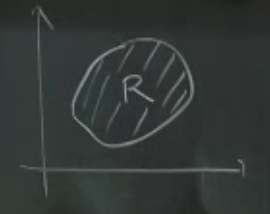
\includegraphics[height=2cm]{17_3.png}

Bazi durumlarda bu hesap tek entegral ile yapilabiliyor, ama cift entegral
ile daha kolay. Soyle

\[ Alan(R) = \int \int_R 1 \ dA \]

Eger cift entegralleri illa hacim olarak gormek istiyorsak, ustteki hesap
yuksekligi 1, baz alani $R$ olan bir ``hacmi'' hesapliyor. Hacim = baz alan
X yukseklik'tir, ama yukseklik 1 oldugu icin, ustteki hesap ayni sadece baz
alanin ne oldugunu hesaplar! Guzel bir cinlik degil mi?

Ya da, diyelim ki yassi / duz bir objenin kutlesini hesaplamak istiyoruz,
ve yogunluk $\delta = kutle / \textit{birim alan}$ olarak verilmis. Her
ufak parca icin kutle

\[ \Delta m = \delta \cdot \Delta A \]

Tum kutleyi ustteki ufak kutleleri toplayarak elde edebiliriz. 

\[ \int \int_R \delta \cdot dA \]

Eger yogunluk objenin her noktasinda ayniysa, $\delta$ degiskenini
formulden cikartabiliriz tabii, ama her $x,y$ noktasinda degisme durumu var
ise, ustteki entegral hesabi guzelce yapacaktir.

2) $R$ bolgesinde $f$'in ortalamasi 

Bir ortalama hesabini normalda, mesela belli sayilar icin, nasil
yapacagimizi biliyoruz. Sayilari aliyoruz, toplamlarini kac sayi olduguyla
boluyoruz. Benzer sekilde, icinde oldugunuz odanin ortalama sicakligini
hesaplamak istesek bir suru noktada sicaklik olcumu alip, onlari toplayip
bolmemiz gerekir. Fakat bu sicaklik olcumu icin potansiyel olarak sonsuz
tane olcum olabilir. Bu hesabin matematiksel sekli olcum fonksiyonunu alan
uzerinden entegre etmek, sonra alan buyukluguyle bolmektir. 

Notasyon

\[ \textit{f'in ortalamasi} = \bar{f} \]

\[ \bar{f} = \frac{1}{Alan(R)} \int \int f \ dA \]

2a) Ustteki ortalama birbicimli (uniform) bir ortalama, her noktaya
ayni onemi veriyoruz. Eger bazi noktalara daha fazla agirlik vermek
istersek, agirlikli ortalama (weighted average) hesabi yapabiliriz.

\[ \textit{f'in agirlikli ortalamasi} = \frac{1}{Kutle(R)} 
\int \int_R f \ \delta \ dA
 \]

Agirlikli ortalama kutle merkezi (center of mass) hesaplarinda ise
yarar. Belki bir objenin bazi taraflari digerlerine gore daha agir, bu
objenin kutle merkez hesabi bunu hesaba katmali. 

2 Boyutta kutle merkezi $(\bar{x},\bar{y})$, 

\[  \bar{x}  = \frac{1}{Kutle} \int \int_R x \ \delta \ dA  \]

\[  \bar{y}  = \frac{1}{Kutle} \int \int_R y \ \delta \ dA  \]


3) Donme direnci (moment of intertia): Bu kavram bir objenin donuse
karsi gosterdigi direnctir, aynen itilmeye karsi direnisin kutle oldugu
gibi. Bir objeyi ne kadar ileri firlatabilecegim onun kutlesine baglidir,
onu ne kadar dondurebilecegim donme direncine baglidir. 

DD hesabi icin bir eksen tanimlanmasi gereklidir, cunku ``neyin etrafinda
donulecegi'' ancak bir eksene gore anlamlidir. Hesap nasil yapilir? 

Ana fikir kinetik enerjiyi kullanmak. Eger noktasal bir kutle $m$ hiz $v$
ile hareket ediyorsa, kinetik enerji $1/2 mv^2$. 

Itmek yerine kutleyi bir eksen etrafinda $r$ uzaklikta $\omega$ rotasyonel
hizda donecek sekilde hareket ettirirsem,

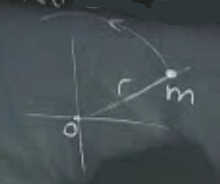
\includegraphics[height=3cm]{17_4.png}

\[ \frac{1}{2}mv^2 = \frac{1}{2}mr^2\omega^2  \]

Donme direncinin itilmeyle olan baglantisi formulde gozukuyor, $m$ itilme
formulunde $v^2$'in katsayisi. $mr^2$ ise $\omega^2$'nin katsayisi.

Fakat bu basit bir noktasal kutle icin. Daha cetrefil bir objeyi dondurmek
istiyorsak, bu objenin tum DD'si objenin icindeki tum noktasal DD'lerin
toplami olacaktir. 

Yogunlugu $\delta$ olan bir obje icin 

\[ \Delta m = \delta \Delta A \]

DD

\[ \Delta m r^2 = r^2 \delta \Delta A \]

Ustteki parcalari bir bolge uzerinden toplarsam, tum DD'yi bulurum. Nihai
formul

\[ I_0 = \int \int_R r^2 \delta \ dA \]

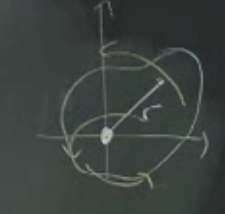
\includegraphics[height=3cm]{17_5.png}

Rotasyonel kinetik enerji $\frac{1}{2}I_0 \omega^2$

Peki diger tur donme hareketleri? Mesela objeyi $x$ ekseni etrafinda da
dondurebilirdim. 

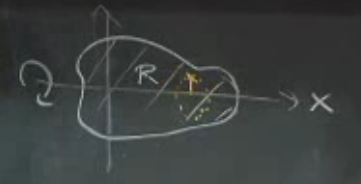
\includegraphics[height=4cm]{17_6.png}

Hesap benzer kavramlari kullanir, donme eksenine olan uzaklik $r$
kullanilir. Ustteki resimde kirmizi noktayi ele alalim, uzakligi kirmizi
okla gosteriliyor. Bu uzaklik aslinda $|y|$ degil midir? $r^2$ lazim, o
zaman $y^2$ kullaniriz. 

\[ I_x = \int \int y^2 \delta dA \]

Ornek

$a$ yaricapindaki bir diski orijin etrafinda dondurmek istiyoruz 

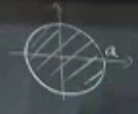
\includegraphics[height=3cm]{17_7.png}

Yogunluk birbicimli (uniform) ve $\delta = 1$. Donme direnci nedir? 

\[ I_0 = \int \int r^2 dA \]

$r$ ne? Insanin icinden hemen $a$ demek gelebilir, ama degil. Unutmayalim,
``her nokta'' icin DD hesapliyoruz, yani disk icindeki her nokta dikkate
alinmali, ve bu noktalarin hepsi $a$ uzakliginda degiller, uzakliklari $\le
a$. 

Kutupsal kordinata gecmek iyi olur mu? Evet. 

\[ = \int_0^{2\pi} \int_0^a r^2 r dr d\theta \]


\[ = 2\pi \frac{a^4}{4} = \frac{\pi a^4}{2} \]

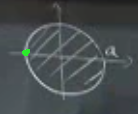
\includegraphics[height=3cm]{17_8.png}

Ya orijin yerine ustteki yesil noktada etrafinda dondurmek isteseydim? Hani
frizbiyi alip parmaginiz etrafinda dondurdugunuzde oldugu gibi. 

Bu hesap icin iki secenek var. Eger kordinat sistemi oldugu gibi kalirsa,
isler biraz zor. Ama sistemi degistirip yesil noktayi yeni orijin haline
getirirsek, isler biraz daha kolay. 

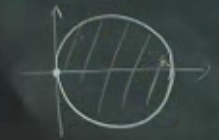
\includegraphics[height=3cm]{17_9.png}

Formul yine ayni

\[ I_0 = \int \int r^2 r dr d\theta \]

Sinirlar nasil hesaplanir? 

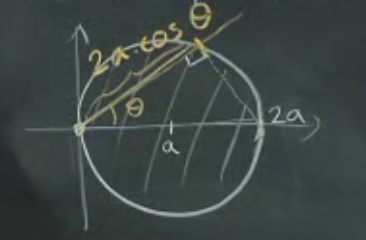
\includegraphics[height=4cm]{17_10.png}

[Yeni] orijinden isin gonderdigimizi dusunelim, bu isinlar cemberden nerede
disari cikar? Yani isaretli yerin uzunlugu nedir? $2a \cos\theta$. Peki
$\theta$ sinirlari nedir? $-\pi$ ile $\pi$, yani $y$ ekseninin tamamen sag
tarafi. ``Ama y ekseni uzerindeyken cembere girip cikmiyoruz'' dusuncesi
akla gelebilir, fakat orada teget halindeyiz, yani sinirlar dogru. 

\[ I_0 = \int_{-\pi/2}^{\pi/2} \int_0^{2a \cos\theta} r^2 r dr d\theta \]

Ic

\[ = \bigg[ \frac{r^4}{4} \bigg]_{0}^{2a \cos\theta} =
4a^4 \cos^4\theta
\]


Dis

\[ I_0 = \int_{-\pi/2}^{\pi/2} 4a^4 \cos^4\theta d\theta \]

Ders Notlari 3B icinde bu formulun cabuk hesabi var. Sonuc

\[  = \frac{3}{2} \pi a^4 \]

Yani bir frizbiyi ortasindan dondurmek yerine kenar noktasi etrafinda
dondurmek 3 kat daha zor. 






















---

Kaynaklar

[1] Bu konu hakkinda Uygulamali Matematik kitapcigimizdaki ``Entegralleri
Nasil Dusunelim'' yazisinin okunmasini da tavsiye ederim. 













\end{document}
